\documentclass[cs4size,a4paper]{ctexart}   
%==================== 数学符号公式 ============
\usepackage{amsmath}                 % AMS LaTeX宏包
\usepackage[style=1]{mdframed}
\usepackage{amsthm}
\usepackage{amsfonts}
\usepackage{mathrsfs}                % 英文花体字 体
\usepackage{bm}                      % 数学公式中的黑斜体
\usepackage{bbding,manfnt}           % 一些图标,如 \dbend
\usepackage{lettrine}                % 首字下沉,命令\lettrine
\def\attention{\lettrine[lines=2,lraise=0,nindent=0em]{\large\textdbend\hspace{1mm}}{}}
\usepackage{longtable}
\usepackage[toc,page]{appendix}
\usepackage{geometry}                % 页边距调整
\geometry{top=3.0cm,bottom=2.7cm,left=2.5cm,right=2.5cm}
%====================公式按章编号==========================
\numberwithin{equation}{section}
\numberwithin{table}{section}
\numberwithin{figure}{section}
%================= 基本格式预置 ===========================
\usepackage{fancyhdr}
\pagestyle{fancy}
\fancyhf{}  
\fancyhead[C]{\zihao{5}  \kaishu 计\ 算\ 机\ 通\ 信\ 与\ 网\ 络\ 实\ 验\ 报\ 告}
\fancyfoot[C]{~\zihao{5} \thepage~}
\renewcommand{\headrulewidth}{0.65pt} 
%\CTEXsetup[format={\centering\bfseries\zihao{-2}}]{section}
\ctexset{
    section={format={\centering\bfseries\zihao{-2}}},
    subsection={nameformat={\bfseries\zihao{3}}},
    subsubsection={nameformat={\bfseries\zihao{4}}}
}
%================== 图形支持宏包 =========================
\usepackage{subfigure}
\usepackage{graphicx}                % 嵌入png图像
\usepackage{color,xcolor}            % 支持彩色文本、底色、文本框等
\usepackage{hyperref}                % 交叉引用
\usepackage{caption}
\captionsetup{figurewithin=section}
%==================== 源码和流程图 =====================
\usepackage{listings}                % 粘贴源代码
\usepackage{xcolor}
\usepackage{color}
\definecolor{dkgreen}{rgb}{0,0.6,0}
\definecolor{gray}{rgb}{0.5,0.5,0.5}
\definecolor{mauve}{rgb}{0.58,0,0.82}
\usepackage{xcolor}
\lstset{
    %行号
    numbers=left,
    %背景框
    framexleftmargin=8mm,
    xleftmargin=2em,
    xrightmargin=2em, 
    aboveskip=1em,
    frame=none,
    %背景色
    %backgroundcolor=\color[rgb]{1,1,0.76},
    backgroundcolor=\color[RGB]{245,245,244},
    %样式
    breaklines=true,
    basicstyle=\footnotesize, 
    keywordstyle=\bf\color{blue},
    identifierstyle=\bf,
    numberstyle=\color[RGB]{0,192,192},
    commentstyle=\it\color[RGB]{0,96,96},
    stringstyle=\rmfamily\slshape\color[RGB]{128,0,0},
    %显示空格
    showstringspaces=false
}


%--------------------
\hypersetup{hidelinks}
\usepackage{booktabs}  
\usepackage{shorttoc}
\usepackage{tabu,tikz}
\usepackage{float}

\usepackage{multirow}



\tabcolsep=1ex
\tabulinesep=\tabcolsep
\newlength\tikzboxwidth
\newlength\tikzboxheight
\newcommand\tikzbox[1]{
    \settowidth\tikzboxwidth{#1}
    \settoheight\tikzboxheight{#1}
    \begin{tikzpicture}
        \path[use as bounding box]
            (-0.5\tikzboxwidth,-0.5\tikzboxheight)rectangle
            (0.5\tikzboxwidth,0.5\tikzboxheight);
        \node[inner sep=\tabcolsep+0.5\arrayrulewidth,line width=0.5mm,draw=black]
            at(0,0){#1};
    \end{tikzpicture}%
}

\makeatletter
\def\hlinew#1{
    \noalign{\ifnum0=`}\fi\hrule \@height #1 \futurelet
    \reserved@a\@xhline
}
   
\newcommand{\tabincell}[2]{\begin{tabular}{@{}#1@{}}#2\end{tabular}}%

\usepackage{subfigure}

\usepackage{ifthen}


\usepackage{graphicx} 
\newcommand{\HRule}{\rule{\linewidth}{0.5mm}}

\newtheorem{Theorem}{定理}
\newtheorem{Lemma}{引理} 
%%使得公式随章节自动编号
\makeatletter
\@addtoreset{equation}{section}
\makeatother
\renewcommand{\theequation}{\arabic{section}.\arabic{equation}}

%-------------------------
	
\usepackage{pythonhighlight}
\usepackage{tikz}                    
\usepackage{tikz-3dplot}
\usetikzlibrary{shapes,arrows,positioning}
%===================   正文开始    ===================
\begin{document}
\bibliographystyle{gbt7714-2005}     %论文引用格式
%===================  定理类环境定义 ===================
\newtheorem{example}{例}              % 整体编号
\newtheorem{algorithm}{算法}
\newtheorem{theorem}{定理}            % 按 section 编号
\newtheorem{definition}{定义}
\newtheorem{axiom}{公理}
\newtheorem{property}{性质}
\newtheorem{proposition}{命题}
\newtheorem{lemma}{引理}
\newtheorem{corollary}{推论}
\newtheorem{remark}{注解}
\newtheorem{condition}{条件}
\newtheorem{conclusion}{结论}
\newtheorem{assumption}{假设}
%==================重定义 ===================
\renewcommand{\contentsname}{目录}     
\renewcommand{\abstractname}{摘要} 
\renewcommand{\refname}{参考文献}     
\renewcommand{\indexname}{索引}
\renewcommand{\figurename}{图}
\renewcommand{\tablename}{表}
\renewcommand{\appendixname}{附录}
\renewcommand{\proofname}{证明}
\renewcommand{\algorithm}{算法} 
%============== 封皮和前言 =================
\begin{titlepage}

\begin{center}


% Upper part of the page

\includegraphics[width=0.65\textwidth]{figure/logo}\\[1cm]    

\textsc{\LARGE Huazhong University of Science and Technology}\\[1.5cm]

\textsc{\Large Lab Report}\\[0.5cm]


% Title
\HRule \\[0.4cm]
{ \huge \bfseries 计算机通信与网络 实验报告}\\[0.4cm]

\HRule \\[1.5cm]

% Author and supervisor

\begin{minipage}{0.4\textwidth}
\large
{\heiti 姓名}\quad 邹雅

{\heiti 学号}\quad U201915035

{\heiti 班级}\quad ACM1901

{\heiti 时间}\quad \today
\end{minipage}

\vfill

\end{center}

\end{titlepage}

\pagestyle{plain}
\pagenumbering{Roman}
\pagestyle{empty}
\tableofcontents 
\thispagestyle{empty}
%============== 论文正文   =================
\pagestyle{fancy}
\pagenumbering{arabic}
\section{实验一\ \ Socket 编程实验}
\subsection{环境}
\subsubsection{开发运行平台}
\setlength{\parindent}{0pt}
开发及运行设备配置:\\
\hspace*{2em}CPU:2.3 GHz Quad-Core Intel Core i5\\
\hspace*{2em}设备OS:macOS BigSur 11.3.1\\
\hspace*{2em}Memory:8 GB 2133 MHz LPDDR3\\
\hspace*{2em}虚拟机:Windows 10 64-bit\\
开发平台:Visual Studio 2019\\
\hspace*{2em}编程语言:C++\\
\subsection{系统功能需求}
\smallskip
\vspace{0.2cm}
编写一个 Web 服务器软件,要求如下:\\
\textbf{基本要求}
\begin{itemize}
  \item 可配置Web服务器的监听地址、监听端口和主目录(不得写在代码里面,不能每配置一次都要重编译代码);
  \item 能够单线程处理一个请求。当一个客户(浏览器,输入 URL:http://202.103.2.3/index.html)连接时创建一 个连接套接字;
  \item 从连接套接字接收http请求报文,并根据请求报文的确定用户请求的网页文件;
  \item 从服务器的文件系统获得请求的文件。 创建一个由请求的文件组成的 http 响应报文;
  \item 经 TCP 连接向请求的浏览器发送响应,浏览器可以正确显示网页的内容;
\end{itemize}
\textbf{高级要求}
\begin{itemize}
  \item 能够传输包含多媒体(如图片)的网页给客户端,并能在客户端正确显示;
  \item 在服务器端的屏幕上输出请求的来源(IP 地址、端口号和 HTTP 请求命令行);
  \item 在服务器端的屏幕上能够输出对每一个请求处理的结果;
  \item 对于无法成功定位文件的请求,根据错误原因,作相应错误提示,并具备一定的异常情况处理能力。
\end{itemize}

\subsection{系统设计}
\hspace*{2em}使用流式套接字进行编程,流式套接字是基于连接的编程,必须先建立连接后,才能从数据流中读出数据。\\
\hspace*{2em}系统分为两个模块:
\begin{itemize}
  \item server服务器模块,负责创建套接字并监听,当连接客户端后通过新的线程将任务交给sessionClient模块处理响应
  \item sessionClient处理请求模块,解析报文并回传响应
\end{itemize}
\hspace*{2em}由流式套接字构造的系统流程如下所述:创建套接字,来用于监听;对监听套接字进行绑定;监听并等待连接;连接成功,生成会话套接字,用于接受客户端发来的数据流并且发送数据;对客户端的请求响应后通过会话套接字发送响应报文及文件;发送完之后关闭套接字。流程图1.1所示。\\

%开始插入图片
\begin{figure}[htbp] % htbp代表图片插入位置的设置
\centering %图片居中
%添加图片;[]中为可选参数,可以设置图片的宽高;{}中为图片的相对位置
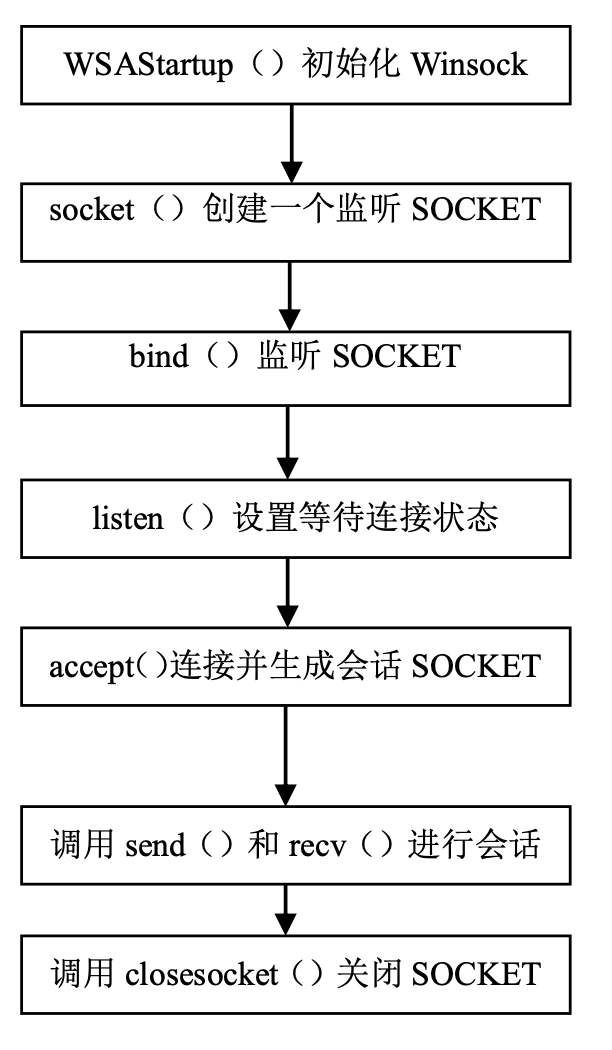
\includegraphics[width=6cm]{Lab Report/figure/图1.1.png}
\caption{服务器端套接字构造流程图} % 图片标题
\end{figure}

\subsection{系统实现}
\subsubsection{server服务器模块}
\hspace*{2em}1.在Windows环境下首先需要初始化winsock,使用WSAStartup函数;如果发生错误输出初始化失败信息并退出该程序,表示后续无法进行服务。\\
\begin{lstlisting}[language=c++]
WSAData wsaData;
int nRc = WSAStartup(0x0202, &wsaData);
if (nRc) {
	cout<<"startup winsock error"<<endl;
	return 0;
}
\end{lstlisting}
\hspace*{2em}2.创建服务器监听套接字,使用数据类型SOCKET,如果创建失败则输出创建失败信息。\\
\begin{lstlisting}[language=c++]
SOCKET srvSocket = socket(AF_INET, SOCK_STREAM, 0);
if (srvSocket == INVALID_SOCKET)
	cout << "create socket error" << endl;
\end{lstlisting}
\hspace*{2em}3.配置Web服务器的监听地址、监听端口和主目录,由于要求这些设置不能写在代码中,不能每配置一次都要重编译代码,所以采用通过在控制台输入信息并读取的方式来进行设置。其中端口号和监听IP地址需要通过一个类型为sockaddr\_in的地址变量绑定在套接字上,使用函数bind,如果绑定失败,则输出监听绑定失败的信息并退出,否则无输出。\\
\begin{lstlisting}[language=c++]
sockaddr_in addr;
int port;
char ip[20],content[20];
cout << "input ip" << endl;  cin >> ip;
cout << "input port" << endl;  cin >> port;
cout << "input content" << endl;  cin >> content;
fileposition = content;//fileposition为全局变量可以给sessionClient传递文件夹位置
addr.sin_family = AF_INET;
addr.sin_port = htons(port);
addr.sin_addr.S_un.S_addr = inet_addr(ip);
//binding
int rtn = bind(srvSocket, (LPSOCKADDR)&addr, sizeof(addr));
if (rtn == SOCKET_ERROR) {
	nSocketError = WSAGetLastError();
	cout << "bind error = " << nSocketError;
	return 0;
}
\end{lstlisting}
\hspace*{2em}从控制台输入IP时,保存为点分十进制的IP地址的字符数组。但是套接字需要的IP地址为二进制无符号长整型,所以需要函数inet\_addr将字符串形式的IP地址转换为unsigned long形式的值。输入端口号在内存中存储的是按电脑的小端存储的,但是网络是大端存储,故需要函数htons把主机字节顺序转换为网络字节顺序。\\
\hspace*{2em}4.此时套接字部分已经创建完成,需要将其配置为等待连接状态,也就是在没有有连接的时候保持监听状态,需要使用listen函数,如果设置失败则输出失败信息并退出,否则无输出。\\
\begin{lstlisting}[language=c++]
rtn = listen(srvSocket, 5);
if (rtn == SOCKET_ERROR) {
	nSocketError = WSAGetLastError();
	cout << "listen error = " << nSocketError;
	return 0;
}
\end{lstlisting}
\hspace*{2em}5.进入循环等待连接状态。首先生成会话套接字,需要通过accept函数连接并且得到客户端的IP地址和端口,如果连接失败则输出失败信息并返回,否则将该会话套接字通过一个新的线程交给sessionClient处理请求模块去处理。由于服务器端需要一直保持打开并监听的状态,等待连接的循环会一直运行。
\begin{lstlisting}[language=c++]
while (true) {
	int length = sizeof(sockaddr);
	sockaddr_in clientaddr;
	SOCKET sessionSocket = accept(srvSocket, (sockaddr *)&clientaddr, &length);
	if (sessionSocket == INVALID_SOCKET) {
		nSocketError = WSAGetLastError();
		cout << "accept session error = " << nSocketError;
		return 0;
	}
	string str(content);
	thread sessionThread(sessionToClient,sessionSocket);
	std::cout << "request IP:" << (int)clientaddr.sin_addr.S_un.S_un_b.s_b1 << "." << (int)clientaddr.sin_addr.S_un.S_un_b.s_b2 << "." << (int)clientaddr.sin_addr.S_un.S_un_b.s_b3 << "." << (int)clientaddr.sin_addr.S_un.S_un_b.s_b4<<endl;
	std::cout << "request port:" << clientaddr.sin_port << endl;
	sessionThread.detach();
}
\end{lstlisting}
\subsubsection{sessionClient处理请求模块}
\hspace*{2em}1.当有客户端的请求报文时,recv函数便会从该套接字中接收并放置到指定的缓存区;
\begin{lstlisting}[language=c++]
char* buf = (char*)malloc(1024 * sizeof(char));
int len = 1024;
int charnum = recv(sessionSocket, buf, len, 0);
if (charnum == SOCKET_ERROR) {
	charnum = WSAGetLastError();
	cout << "error" << endl;
	return;
}
\end{lstlisting}
\hspace*{2em}2.对接收到的消息进行解析,这里使用正则表达式进行匹配并获取请求报文中对应的信息。
\begin{lstlisting}[language=c++]
const char* REQERROR = "HTTP/1.1 400 Bad Request\r\n";
//对接受到的消息进行解析
smatch strmatch;//正则表达式结果文本
regex regulation("([A-Za-z]+) +(.*) +(HTTP/[0-9][.][0-9])");//正则表达式规则
string str(buf);//需要用正则表达式的原始文本
int match = regex_search(str, strmatch, regulation);
if (match == 0) {//匹配成功返回1,失败返回0
	cout << "request message error"<<endl;
	sendre = send(sessionSocket, REQERROR, strlen(REQERROR), 0);
	closesocket(sessionSocket);
	return;
}
\end{lstlisting}
\hspace*{2em}匹配成功后再解析得到请求方法和请求文件的url。接着进一步进行正则匹配得到当前请求的文件类型。
\begin{lstlisting}[language=c++]
map<string, string> content_type = {
	{".png", "image/png"},
	{".jpg", "image/jpeg"},
	{".jpeg", "image/jpeg"},
	{".html", "text/html"}
};
string msg_get = strmatch[1];//请求方法
string msg_url = strmatch[2];//请求文件的url
smatch filetype;
regex regulation2("\\..*");
match = regex_search(msg_url, filetype, regulation2);
if (match == 0) {
	std::cout << msg_get + msg_url + "\nFORMAT ERROR\n";
	sendre = send(sessionSocket, REQERROR, strlen(REQERROR), 0);
	closesocket(sessionSocket);
	return;
}
string file_type = filetype[0];
\end{lstlisting}
\hspace*{2em}根据文件夹地址和文件的url进行查找文件,如果没有找到文件则发送NotFound响应报文。
\begin{lstlisting}[language=c++]
const char* NOTFOUND = "HTTP/1.1 404 Not Found\r\n";
ifstream f(fileposition + msg_url, std::ios::binary);
if (!f) {//没有找到文件
	cout << msg_url + "\nNOT FOUND"<<endl;
	sendre = send(sessionSocket, NOTFOUND, strlen(NOTFOUND), 0);
	closesocket(sessionSocket);
	return;
}
\end{lstlisting}
\hspace*{2em}3.读取文件中的内容并得到文件的size,如果size小于等于0的话则响应请求错误。当size正常时,则按照文件内容发送响应报文。这里有一点就是加入长度超过了一个报文可以承载的容量时则分多个报文进行响应。\\
\hspace*{2em}其中HTTP响应报文可以如下例子所示:\\
%开始插入图片
\begin{figure}[htbp] % htbp代表图片插入位置的设置
\centering %图片居中
%添加图片;[]中为可选参数,可以设置图片的宽高;{}中为图片的相对位置
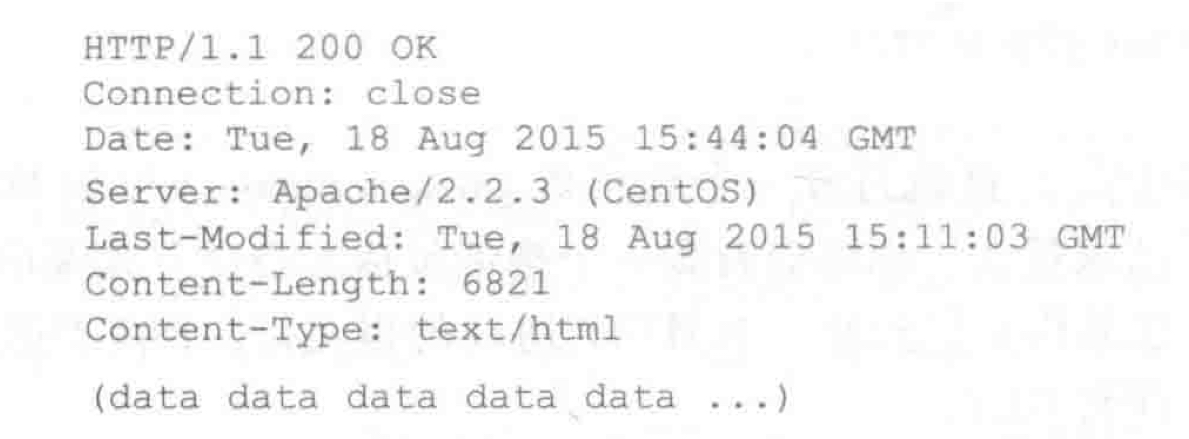
\includegraphics[width=12cm]{Lab Report/figure/image2.jpeg}
\caption{HTTP响应报文例子} % 图片标题
\end{figure}
\begin{lstlisting}[language=c++]
std::filebuf* tmp = f.rdbuf();
int size = tmp->pubseekoff(0, f.end, f.in);
tmp->pubseekpos(0, f.in);
if (size <= 0) {
	sendre = send(sessionSocket, REQERROR, strlen(REQERROR), 0);
	closesocket(sessionSocket);
	return;
}else {
	string Content_Type = content_type[file_type];
	char* buffer = new char[size];
	char* tail = buffer + size;
	tmp->sgetn(buffer, size);
	f.close();
	cout << "successfully get file " + msg_url<<endl;
	stringstream remsg;
	remsg << "HTTP/1.1 200 OK\r\n" << "Connection:close\r\n"<<"Server:Zou Ya\r\n" << "Content Length:" << size	<< "\r\n" << "Content Type:" + Content_Type << "\r\n\r\n";
	string remsgstr = remsg.str();
	const char* remsgchar = remsgstr.c_str();
	int tmpsize = strlen(remsgchar);
	sendre = send(sessionSocket, remsgchar, tmpsize, 0);
	while (buffer < tail) {
		sendre = send(sessionSocket, buffer, size, 0);
		buffer = buffer + sendre;
		size = size - sendre;
	}
	closesocket(sessionSocket);
	return;
}
\end{lstlisting}
\subsection{系统测试及结果说明}
\hspace*{2em}1. 配置Web服务器的监听地址、监听端口和主目录\\
%开始插入图片
\begin{figure}[H] % htbp代表图片插入位置的设置
\centering %图片居中
%添加图片;[]中为可选参数,可以设置图片的宽高;{}中为图片的相对位置
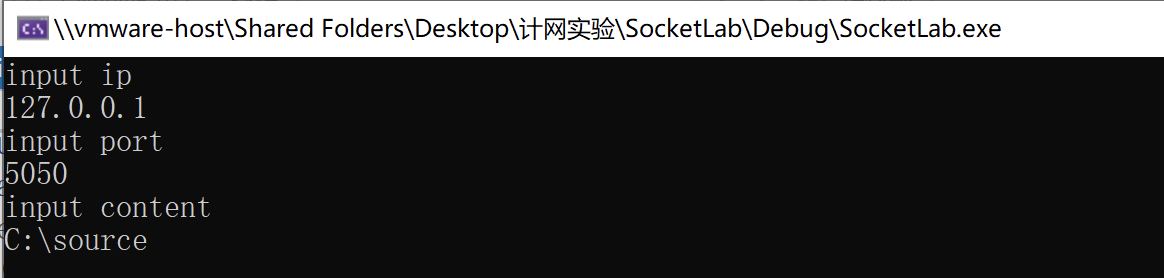
\includegraphics[width=12cm]{Lab Report/figure/image1.3.png}
\caption{配置Web服务器} % 图片标题
\end{figure}

\hspace*{2em}2. 能够开启多个线程处理请求报文。从连接套接字接收http请求报文,并根据请求报文的确定用户请求的网页文件;从服务器的文件系统中获得请求的文件。 创建由请求的文件组成的http响应报文;经TCP连接向请求的客户端发送响应,并且浏览器可以正确显示网页的内容。\\
%开始插入图片
\begin{figure}[H] % htbp代表图片插入位置的设置
\centering %图片居中
%添加图片;[]中为可选参数,可以设置图片的宽高;{}中为图片的相对位置
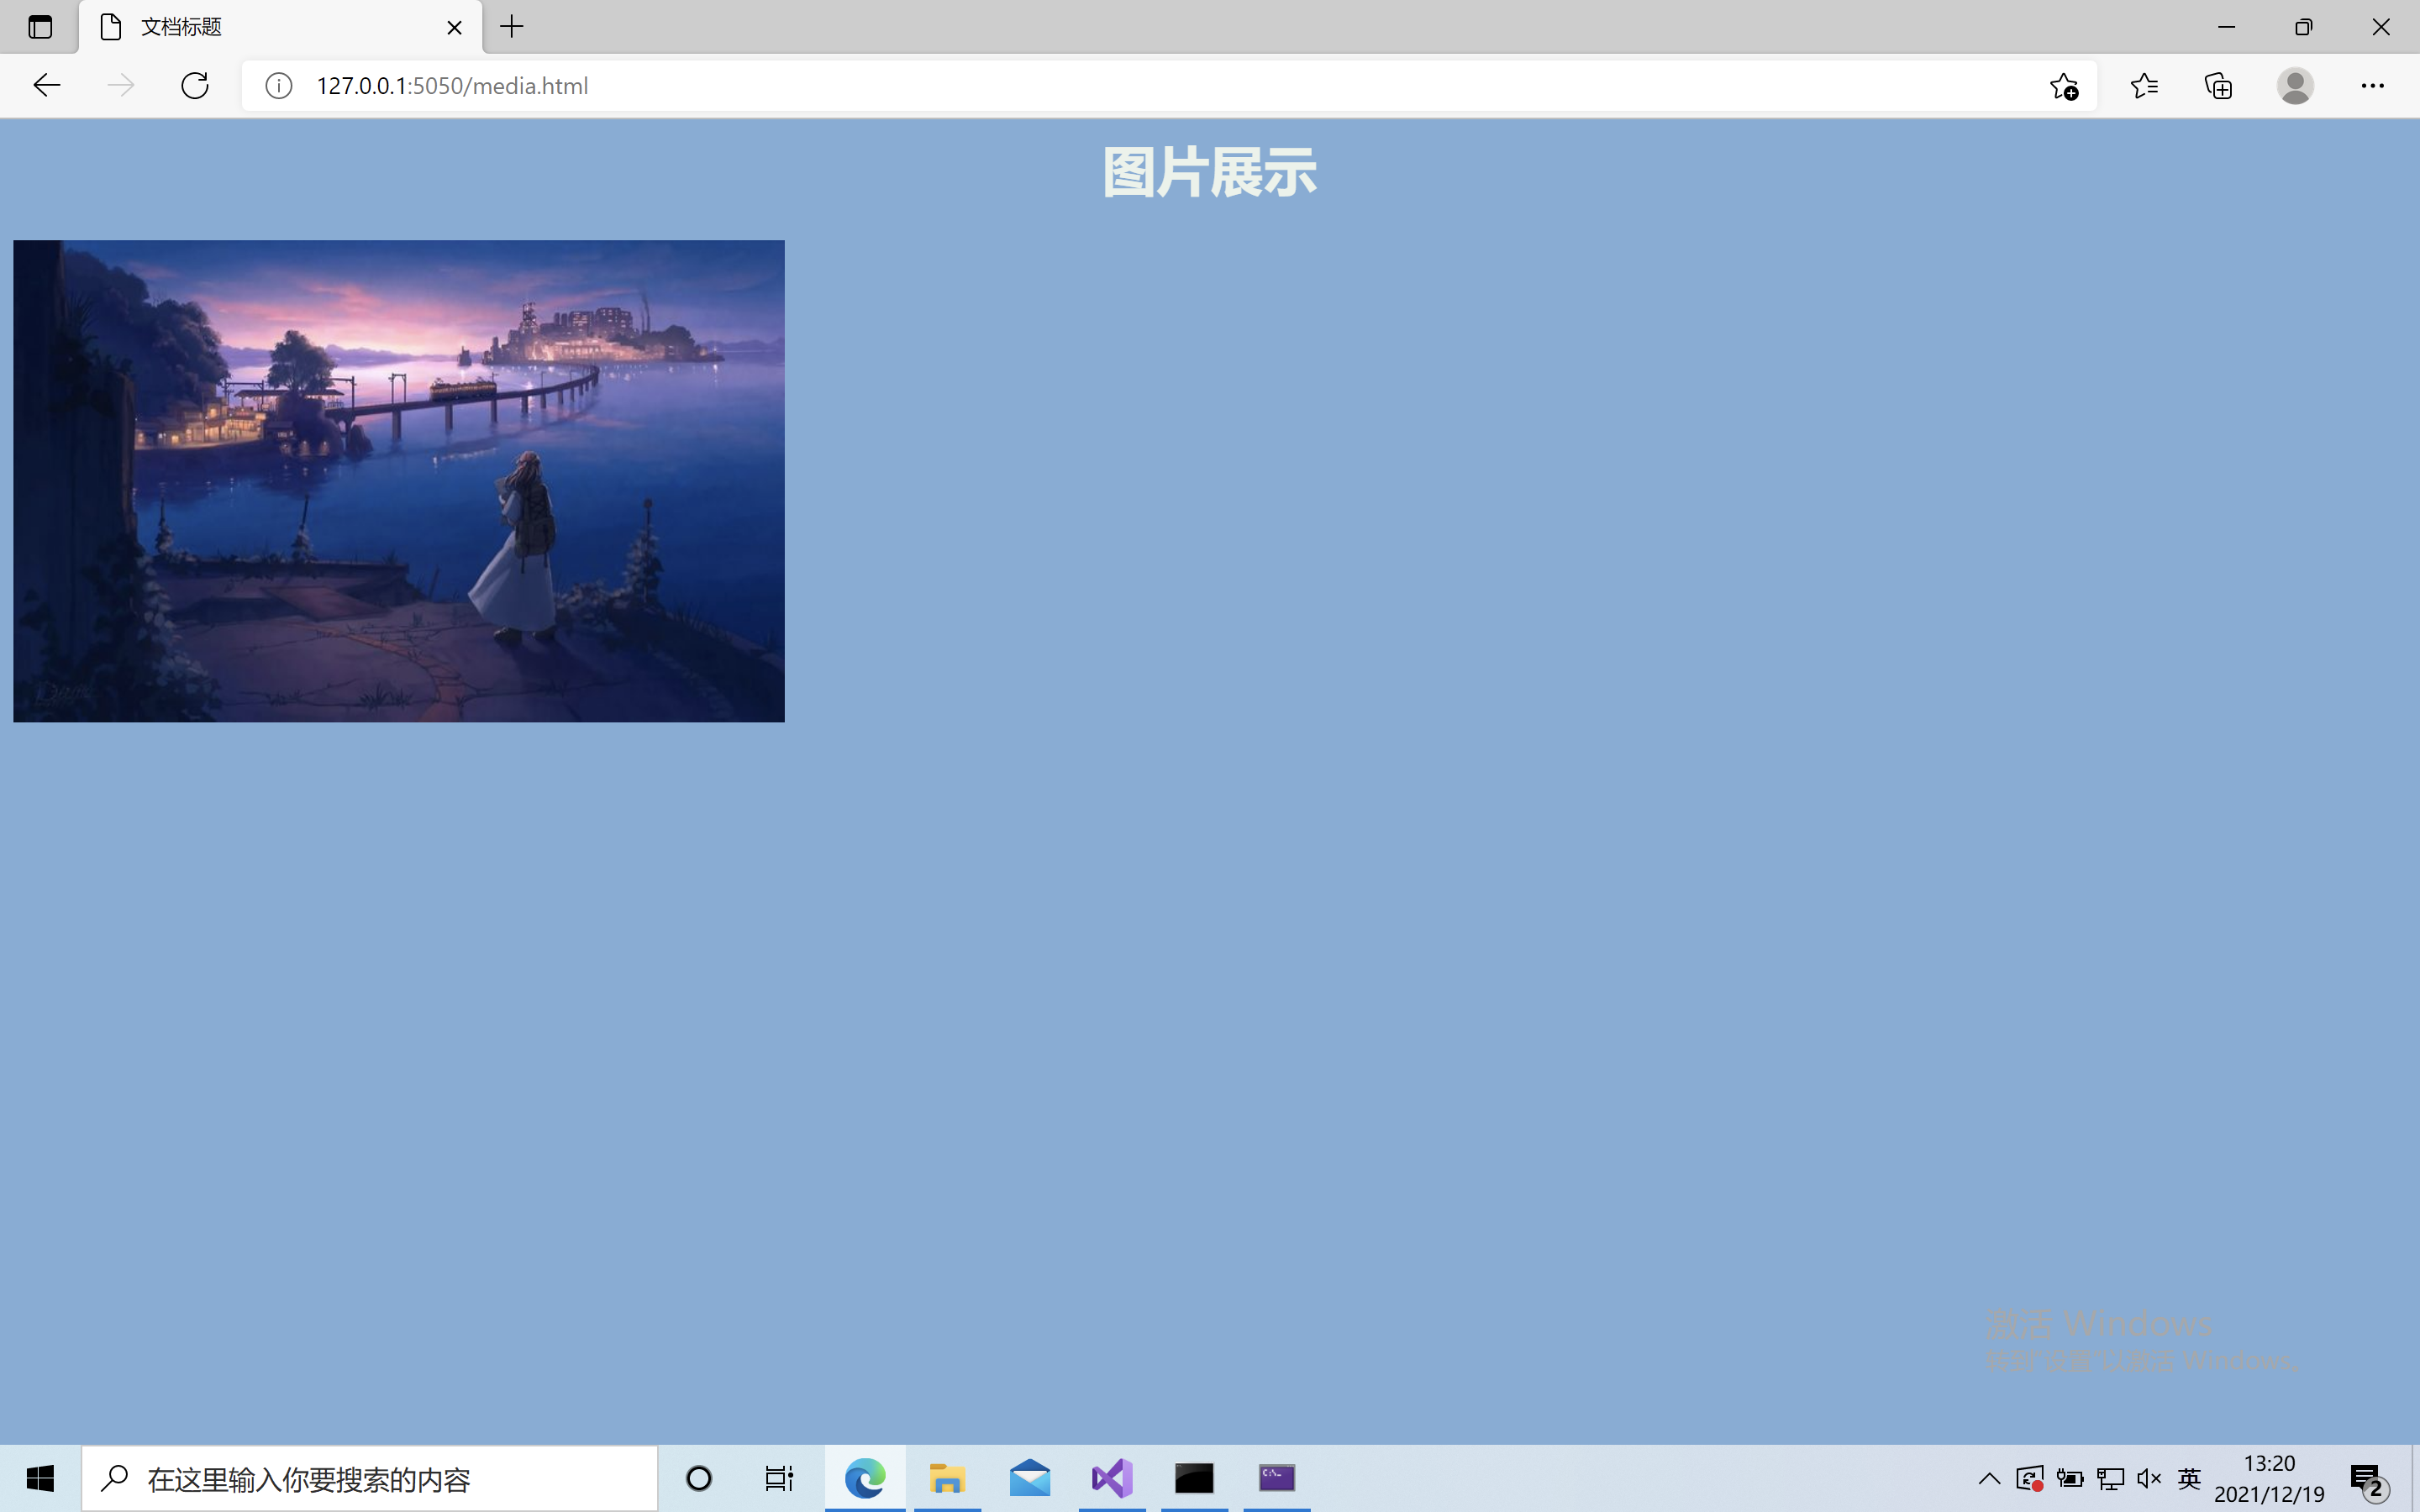
\includegraphics[width=8cm]{Lab Report/figure/image1.4.png}
\caption{浏览器显示网页} % 图片标题
\end{figure}
%开始插入图片
\begin{figure}[H] % htbp代表图片插入位置的设置
\centering %图片居中
%添加图片;[]中为可选参数,可以设置图片的宽高;{}中为图片的相对位置
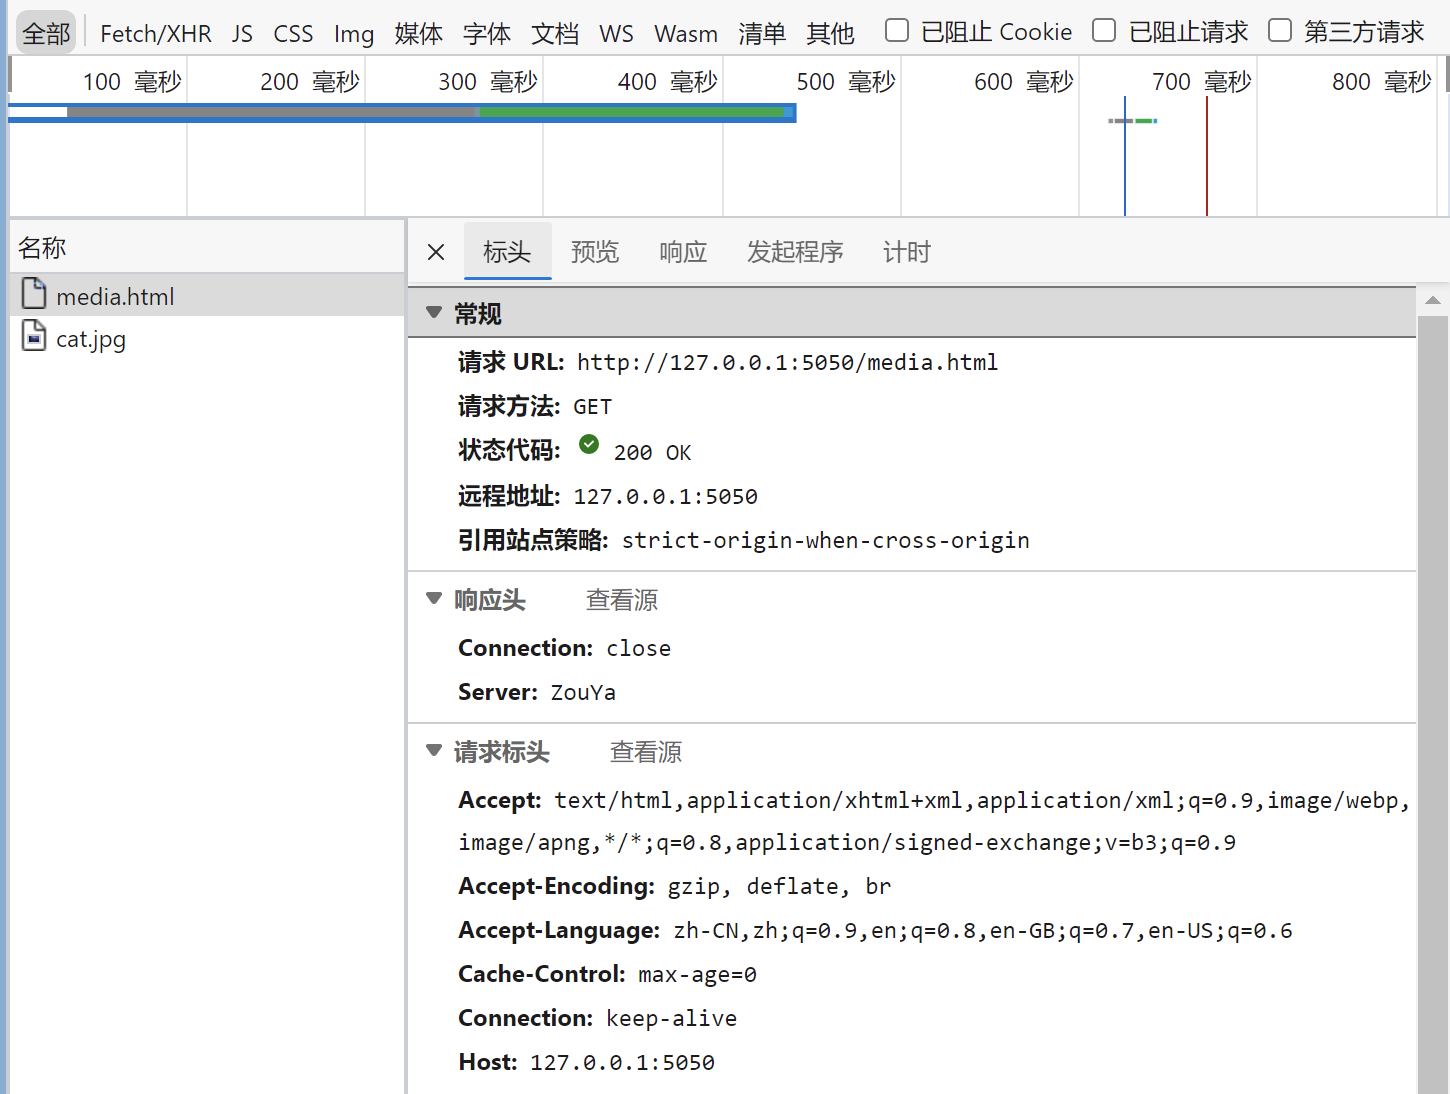
\includegraphics[width=8cm]{Lab Report/figure/image1.5.png}
\caption{浏览器请求和响应报文} % 图片标题
\end{figure}
\hspace*{2em}3. 在服务器端的屏幕上输出请求的来源(IP地址、端口号和HTTP请求命令行)\\
%开始插入图片
\begin{figure}[H] % htbp代表图片插入位置的设置
\centering %图片居中
%添加图片;[]中为可选参数,可以设置图片的宽高;{}中为图片的相对位置
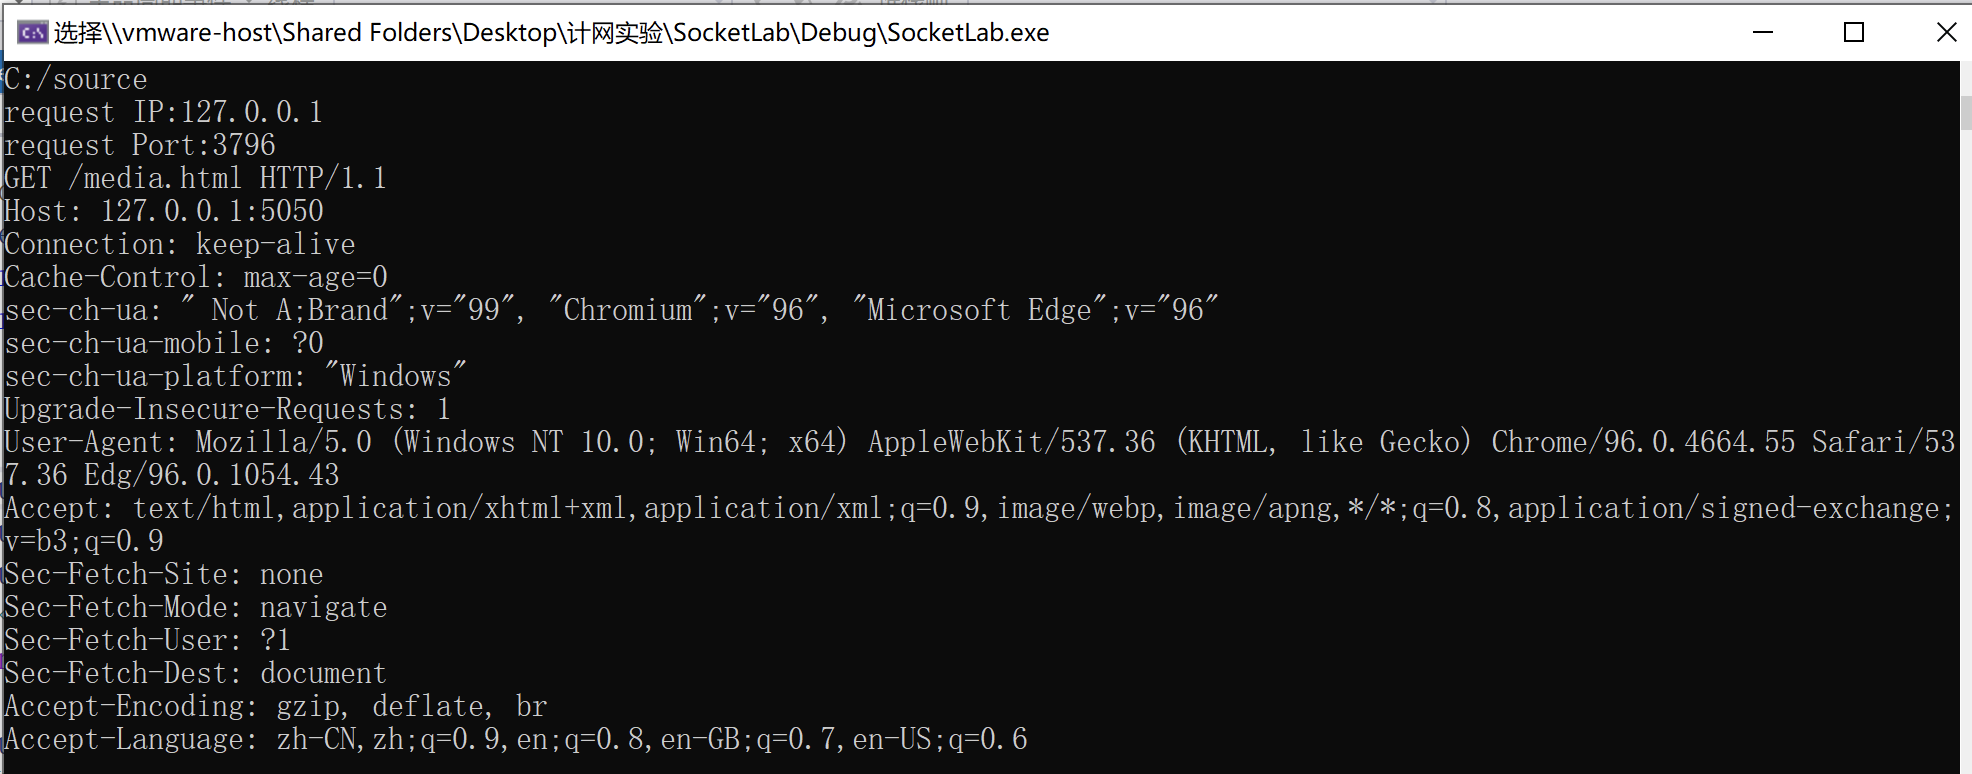
\includegraphics[width=12cm]{Lab Report/figure/image1.6.png}
\caption{控制台输出} % 图片标题
\end{figure}
\hspace*{2em}4.对于无法成功定位文件的请求,根据错误原因,作相应错误提示,并具备一定的异常情况处理能力。\\
%开始插入图片
\begin{figure}[H] % htbp代表图片插入位置的设置
\centering %图片居中
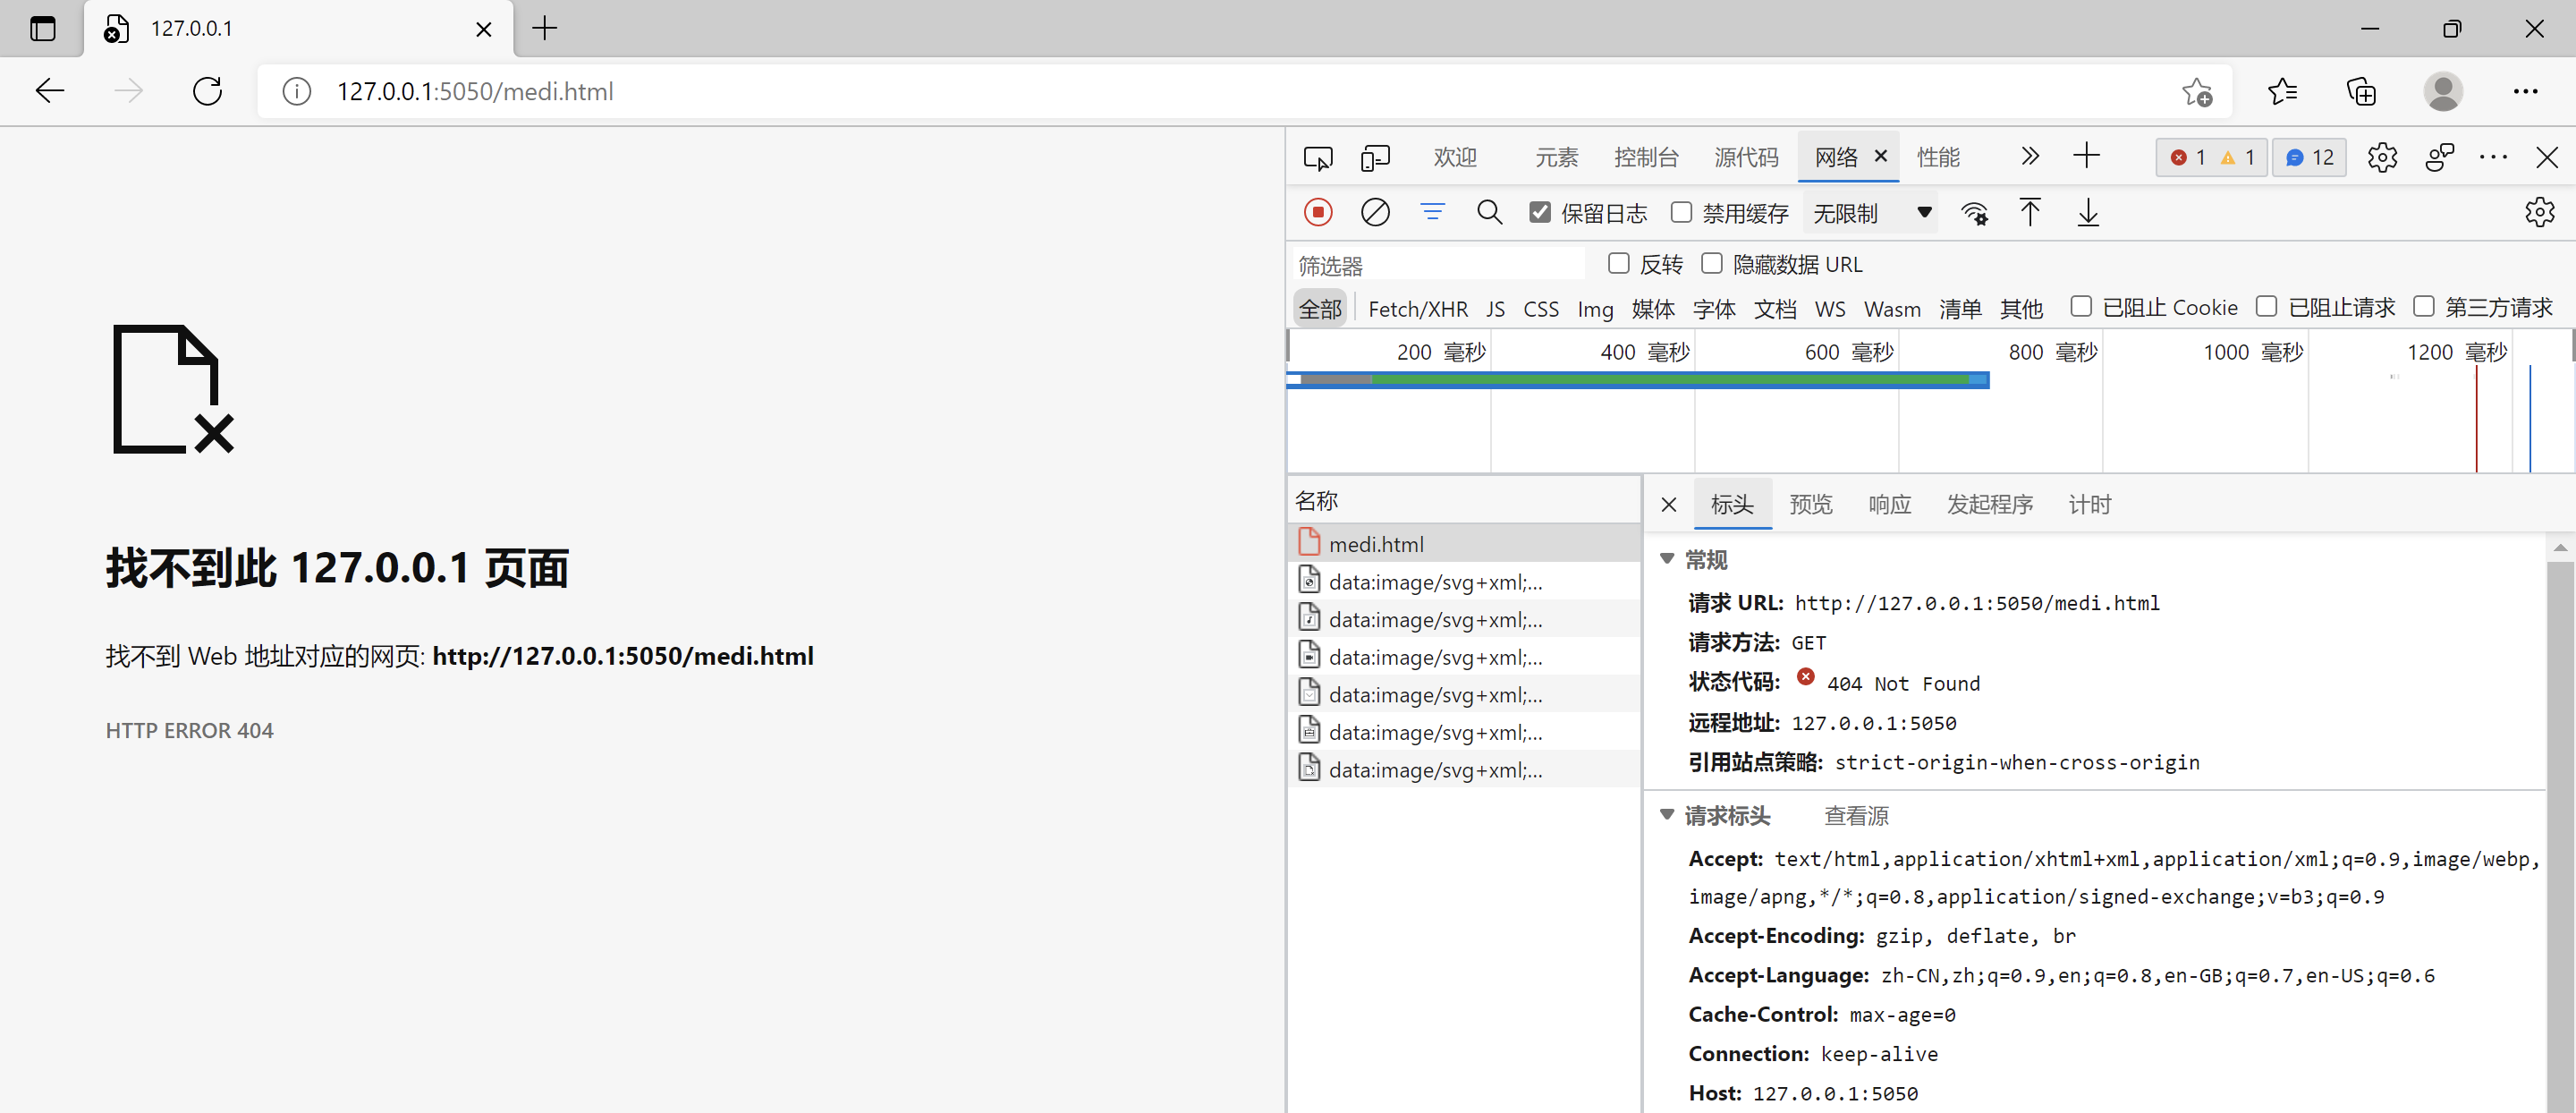
\includegraphics[width=12cm]{Lab Report/figure/image1.7.png}
\caption{无法找到网页时浏览器的显示} % 图片标题
\end{figure}
%开始插入图片
\begin{figure}[H] % htbp代表图片插入位置的设置
\centering %图片居中
%添加图片;[]中为可选参数,可以设置图片的宽高;{}中为图片的相对位置
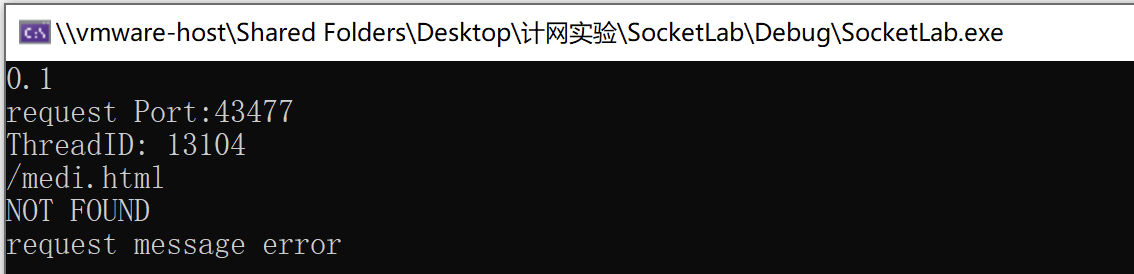
\includegraphics[width=12cm]{Lab Report/figure/image1.8.png}
\caption{无法找到网页时控制台的输出} % 图片标题
\end{figure}
\subsection{其他需要说明的问题}
\hspace*{2em}开始做实验时,不知道怎么处理解析请求报文,后来再网上浏览找到了正则表达式的方法,这是一种十分简洁且方便的处理字符串的方法。

\section{心得体会与建议}
\subsection{心得体会}
\hspace*{2em}在 Socket 编程实验中,通过自己编写代码真正实现服务器端处理客户端的 HTTP 请求,学到了很多,也和我们日常上网的体验相联系起来。\\
\hspace*{2em}在上课的过程中,我们学习了关于 Socket 以及 HTTP 协议的理论知识,了解了理论知识在一定程度上也对网络请求以及响应有了了解,但是刚开始做实验的时候还是有一种很难着手去做的感觉。在明白了是以自己设备的文件系统作为服务器,并用自己的浏览器作为客户端去进行访问,而访问的IP就是本机IP之后,对整个实验有了一个框架性的理解,至少可以开始着手写了。\\
\hspace*{2em}后来看了老师给的文档,对于 Windows 平台下网络通信协议的开发接口 Winsock 的API有了大致的了解,大概知道整个系统应该从哪开始和怎么构建。接下来难题变成了自己怎么去解析请求报文。一开始我打算自己根据 HTTP 请求头来进行解析,但是失败了。然后找到了正则表达式的解析方式,这就十分轻松简易了。\\
\hspace*{2em}第二次和第三次的实验相比起来没有第一次那样无从下手的感觉。第二次的可靠传输协议在老师给的停等协议的基础上,理解了GBN、SR和TCP的原理就可以模仿着写出来了。第三次实验图形化的界面有一种做 Logisim 实验的感觉,把路由器、交换机等等硬件模拟出来,那些看不到的信息配置也通过图形化界面让我们可以直接输入接触到,感觉很有意思。\\
\subsection{建议}
\hspace*{2em}在实验中都给了很详细的 API 说明文档,这对写代码很有帮助,这样我们就不用上网去找查 API 了。但是如果能把这个实验总体要达到的效果告诉我们,比如实验一中要用浏览器模拟客户端,我们对实验有一个大体的认识就不会产生无从下手的感觉了。\\
\hspace*{2em}总体而言,像实验一和实验三这样贴近生活的实验,做起来还是很有意思的。\\
%============= 参考文献 =====================
\addcontentsline{toc}{section}{参考文献}
\begin{thebibliography}{99}  
\bibitem{ref1} James F. Kurose, Keith W. Ross. 计算机网络: 自顶向下方法 (第7版) [M]. 机械工业出版社, 2018.
\end{thebibliography}
\clearpage
%=============  致谢  ======================
\include{body/appendices}

\end{document}
%%%%%%%%%% 结束 %%%%%%%%%%